\documentclass[final,12pt,twoside]{mcthesis}

\usepackage{pstricks}
\usepackage{epsf}
\usepackage{epsfig}
\usepackage{ulem}
\usepackage{hhline}
\usepackage{multirow}
\usepackage{amsmath}
\usepackage{amsfonts}
\usepackage{graphicx} 
\usepackage{fancyhdr}

\begin{document}

\sloppy
\frontmatter
\thesistitle{warning document title undefined}
\shorttitle{warning doc title undefined}
\thesisauthor{FanFan Huang} 
\thesisdegree{M.A.Sc}
\thesisauthprevdeg{B.Eng}
\thesisauthprevdeguni{McMaster University}
\thesissupervisor{Dr. Martin von Mohrenschildt}
\thesisdate{\today}

\makepretitle
\maketitle

%list of custom definitions
\newcommand{\imgsmall}{100px}
\newcommand{\imgmedsmall}{120px}
\newcommand{\imgmedphoto}{200px}
\newcommand{\imgmedium}{300px}



%\dsp
\addcontentsline{toc}{chapter}{Abstract}
%\input{./Chapters/absctract.tex}
\newpage
\addcontentsline{toc}{chapter}{Acknowledgements}
%\input{./Chapters/acknowledge.tex}
\tableofcontents
\listoftables
\listoffigures

\label{pre end}
\mainmatter

\part{Semantics}

%introduction to ladder logic

\chapter{Introduction to Ladder Logic}
\section{Background of Ladder Logic}
\label{section:ladderlogic}

%docment link: http://www.plcs.net/chapters/whatis1.htm
%reasons for development
Ladder logic was originally developed to replace physical relays in PLC's.
As a result the ``language'' resembles a circuit diagram. The left most
and right most ``rung'' represent power rails analogous to GND and VCC what's
placed in between those rungs is the load components /cite{ebookmorris}. In 
the case of programming the entire logic is created from loads you place 
inside these power rails. 

Several other conventions are also observed, power always flows from left 
to right along each rung. Power also flows from top to bottom along the 
rails. This is counter intuitive since ladder logic is suppose to be 
analogous to a circuit schematic and there is no implicit
ordering in circuits. In addition each run must start with inputs and end
with at least one output. Any device that is on a rung is shown in its
initial position.

Modern PLC's operate more like a traditional micro controller and thus the 
original schematic based language can prove to be awkward to work with.

The inputs in ladder are referred to as a load and represented by the 
symbol $-\vert ~ ~ \vert-$. %need reference from tutorial
Loads are boolean values and can be a negated input using the $-\vert/\vert-$ symbol. 
In addition an address is usually assigned to each input referring to 
which port on the physical PLC the input is connected to. Logical and 
can be formed by having two logical loads on one rung \cite{ebookmorris}. 
Similarly logical or can be formed by creating a branch along one 
rung as shown in figure. %figure # %refer to figure here

We can define the language of Ladder Logic as follows $Q = \langle M,S,C,F,R,P \rangle $

\begin{itemize}
	\item M: set of monitored variables.
	\item S: set of state variables.
	\item C: set of controlled outputs.i
	\item R: set of rungs.
	\item P: set of power rails.
\end{itemize}

\begin{figure}[htp]
    \centering
    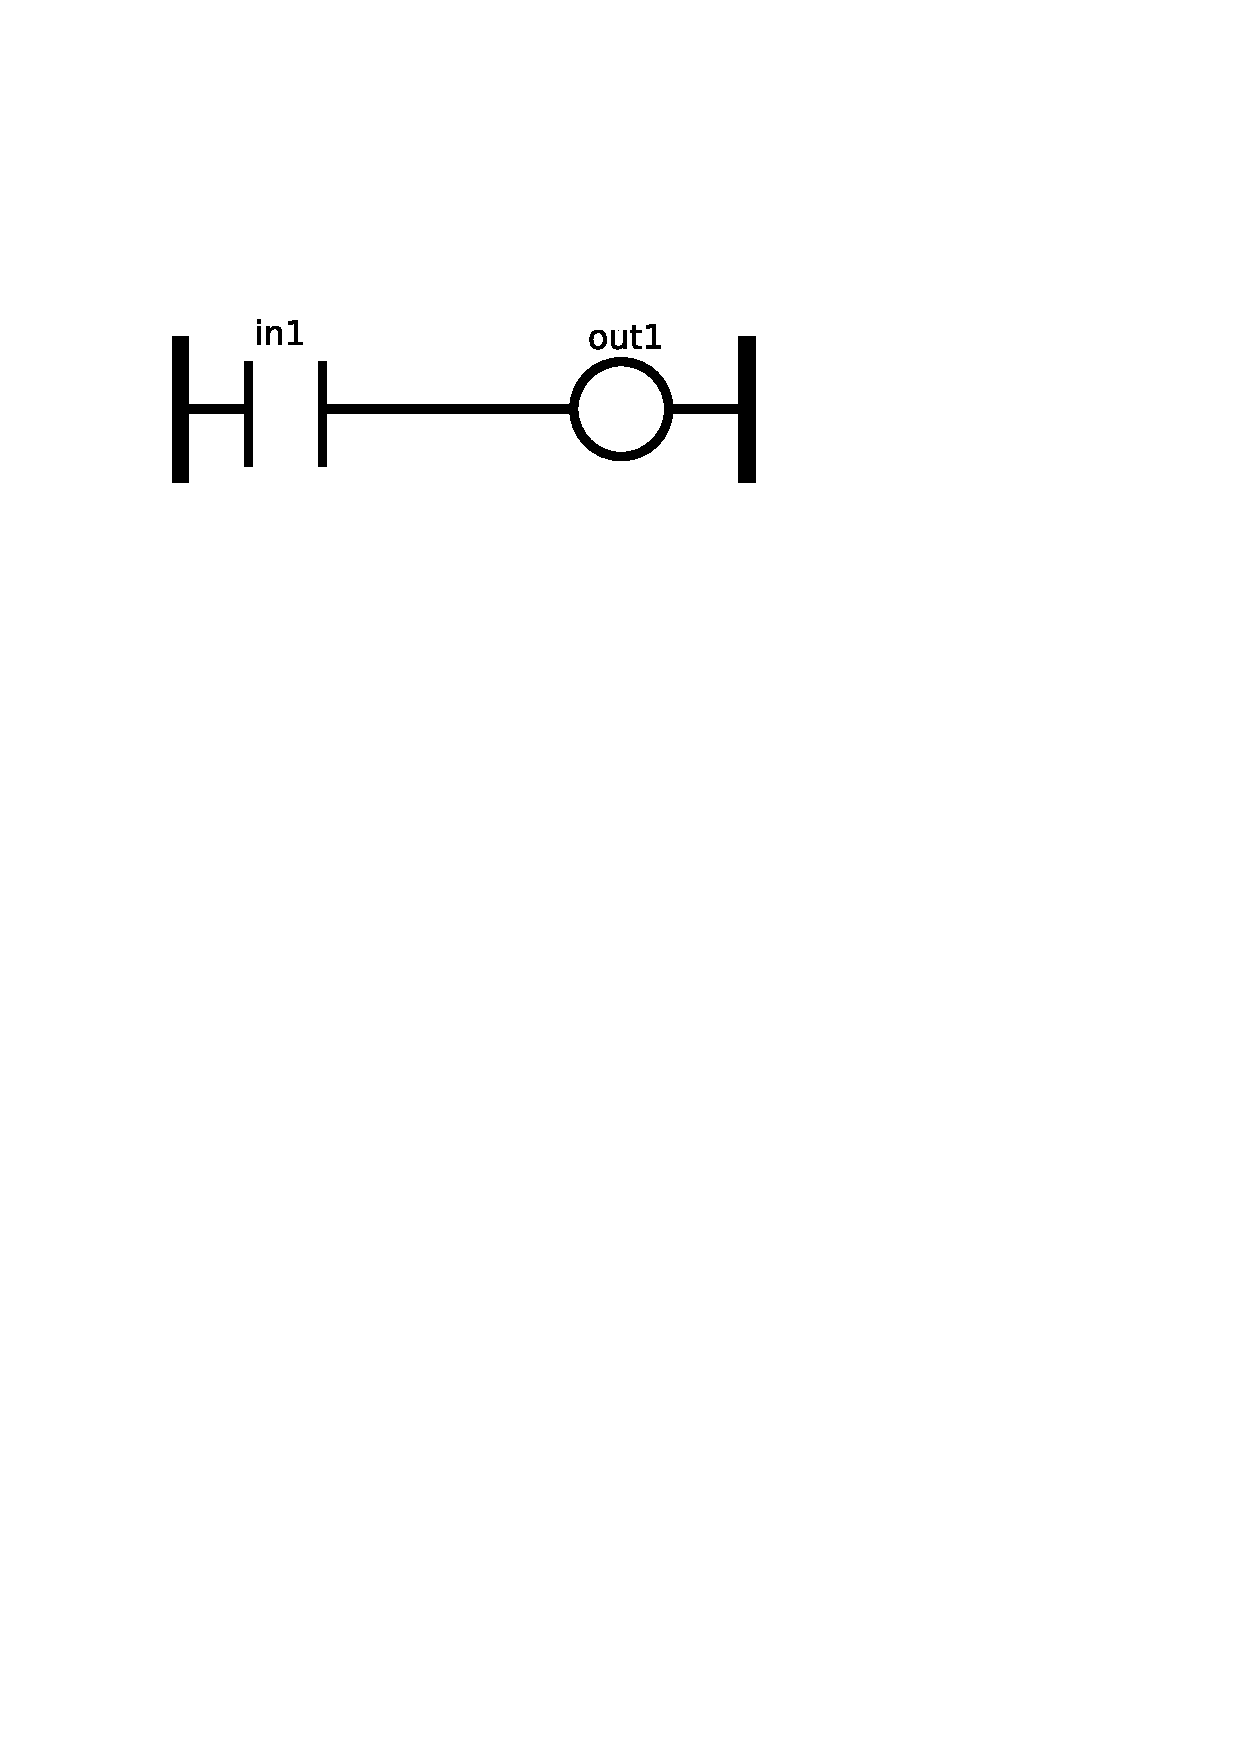
\includegraphics[width=\imgsmall]{./images/intro_fig1.png}
    \caption{Basic Ladder Logic Diagram}
    \label{fig:intro_fig1}
\end{figure}

The most basic structure of ladder logic is shown in figure \ref{fig:intro_fig1}. 
We have 
$$M=\lbrace in_1 \rbrace, S=\lbrace out_1 \rbrace, C=\lbrace out_1 \rbrace, R=\lbrace rung_1 \rbrace, P=\lbrace L,R \rbrace.$$
Note that $rung_1$ is not explicitly labelled in ladder logic but we give it a name here
so we may demonstrate our language framework.

The semantics of figure \ref{fig:intro_fig1} is then: 
\begin{table}[htp]
    \centering
    \begin{tabular}{|l|l|l|}
        \hline
        Action & Result \\
        \hline
        $@T(in_1 = true)$ & $out_1 := true$ \\
        \hline
        $@T(in_1 = false)$ & $out_1 := false$ \\
        \hline
    \end{tabular}
    \caption{Semantics for Fig \ref{fig:intro_fig1}}
    \label{table:table_for_fig1}
\end{table}


Where $@T(<condition>)$ is used to denote the positive edge of a condition becoming true.
We also assume negligible delay between the action occurring and the result being asserted.
It is important to note that our function table must be complete that is have an entry for
all possible combinations in the input domain.

\begin{figure}[htp]
    \centering
    \includegraphics[width=\imgsmall]{./images/intro_fig2.png}
    \caption{Simple AND Logic Diagram}
    \label{fig:intro_fig2}
\end{figure}

When multiple actions are connected on the same rung it is interpreted as a logical AND 
expression. In figure \ref{fig:intro_fig2} we can expand our model to:

$$M=\lbrace in_1, in_2 \rbrace, S=\lbrace out_1 \rbrace, C=\lbrace out_1 \rbrace, R=\lbrace rung_1 \rbrace, P=\lbrace L,R \rbrace.$$

We can see that both $in_1$ and $in_2$ are on $rung_1$. This is interpreted as follows:

\begin{table}[htp]
    \centering
       \begin{tabular}{|l|l|l|}
        \hline
        Action & Result \\
        \hline
        $Initial$ & $in_1 := false, in_2 := false, out_1 := false$\\
        \hline
        $@T(in_1 = true \wedge in_2 = true)$ & $out_1 := true$ \\
        \hline
        $@T(in_1 = false \vee in_2 = false)$ & $out_1 := false$ \\
        \hline
    \end{tabular}
    \caption{Semantics for Fig \ref{fig:intro_fig2}}
    \label{table:table_for_fig2}
\end{table}

The conditions $in_1$ and $in_2$ are combined to form our composed action $@T(in_1 = true \wedge in_2 = true)$ 
as seen in table \ref{table:table_for_fig2}. We also note that there is no action for each individual condition
becoming true nor do we need to individually calculate the timing on $in_1$ or $in_2$ individually.

\begin{figure}[htp]
    \centering
    \includegraphics[width=\imgsmall]{./images/intro_fig3.png}
    \caption{Branching Rungs}
    \label{fig:intro_fig3}
\end{figure}


In addition to multiple actions connected to the same rung, actions can also be branched. A branched rung as
show in figure \ref{fig:intro_fig3} behaves like a logical OR. In addition two or more rungs can be joined
as show in figure \ref{fig:intro_fig3a}. The semantics are equivalent in both figure \ref{fig:intro_fig3} and 
figure \ref{fig:intro_fig3a}.

\begin{figure}[htp]
    \centering
    \includegraphics[width=\imgsmall]{./images/intro_fig3a.png}
    \caption{Branching Rungs (Alternative)}
    \label{fig:intro_fig3a}
\end{figure}

\begin{table}[htp]
    \centering
       \begin{tabular}{|l|l|l|}
        \hline
        Action & Result \\
        \hline
        $Initial$ & $in_1 := false, in_2 := false, out_1 := false$\\
        \hline
        $@T_n(in_1 = true \vee in_2 = true)$ & $out_1 := true$ \\
        \hline
        $@T_n(in_1 = false \wedge in_2 = false)$ & $out_1 := false$\\
        \hline
    \end{tabular}
    \caption{Semantics for Fig \ref{fig:intro_fig3} and Fig \ref{fig:intro_fig3a}}
    \label{table:table_for_fig3}
\end{table}

Since the semantics are the same for both figure \ref{fig:intro_fig3} and figure \ref{fig:intro_fig3a} we can
express both outcomes with function table \ref{table:table_for_fig3}.
As before in table \ref{table:table_for_fig2} in table \ref{table:table_for_fig3} $in_1$ and $in_2$ are composed to form our composed action $@T(in_1 = true \vee in_2 = true)$. However it is also possible to represent this action another way.

\begin{table}[htp]
    \centering
       \begin{tabular}{|l|l|l|}
        \hline
        Action & Result \\
        \hline
        $Initial$ &$in_1 := false, in_2 := false, out_1 := false$\\
        \hline
        $@T(in_1 = true)$ & $out_1 := true$ \\
        \hline
        $@T(in_2 = true)$ & $out_1 := true$ \\
        \hline
        $@T(in_1 = false \wedge in_2 = false)$ & $out_1 := false$\\
        \hline
    \end{tabular}
    \caption{Semantics for Fig \ref{fig:intro_fig3} and Fig \ref{fig:intro_fig3a}}
    \label{table:table_for_fig3a}
\end{table}

In table \ref{table:table_for_fig3a} we choose to represent $in_1$ and $in_2$ as separate actions. This matches figure
\ref{fig:intro_fig3a} more closely but also makes any verification harder than table \ref{table:table_for_fig3}. For
smaller examples table \ref{table:table_for_fig3} make more sense since you can verify relatively simple smaller functions
quite fast. If a system becomes reasonably large however there might be motivation to use the style shown in 
table \ref{table:table_for_fig3a} since it will allow more complex functions to be decomposed into simpler actions.
Since semantically the two are equivalent this paper will focus to the first convention.




%not sure if I should put rung definition here
\pagebreak[4]

\begin{figure}[htp]
    \centering
    \includegraphics[trim= 0 140mm 40mm 10mm, clip, width=\imgmed]{./images/intro_and_graph.pdf} %custom size
    \caption{State diagram conversion for table \ref{table:table_for_fig2}}
    \label{fig:intro_and_graph}
\end{figure}

A rung can be defined as a directed acyclic graph with exactly one source and one sink. The state variables form guard conditions along the edges. A branch in this case represents 2 edges leaving one node. For example figure \ref{fig:intro_fig2}
can be easily converted into a state diagram by observing the results in table \ref{table:table_for_fig2}. 
Each row of table \ref{table:table_for_fig2} is directly converted into an edge with the appropriate guard conditions.
Each output assertion is given their own state. Finally in figure \ref{fig:intro_and_graph} we observe 1 source for the
graph being the start state of the rung, and one sink for the graph being the end state for the rung. We can equivalently take figure \ref{fig:intro_fig3} observe its function table \ref{table:table_for_fig3} and produce an equivalent state digram from its function table.

\pagebreak[3]

\begin{figure}[htp]
    \centering
    \includegraphics[trim= 00mm 140mm 40mm 10mm, clip, width=\imgmed]{./images/intro_or_graph.pdf} %custom size
    \caption{State diagram conversion for table \ref{table:table_for_fig3}}
    \label{fig:intro_or_graph}
\end{figure}

Thus, each rung can be converted into an equivalent state diagram by examining its 
function table, assigning the state variables to guard conditions, and creating a
state for each of the outputs. For completeness we complete this procedure to produce
a state diagram equivalent representation for figure \ref{fig:intro_fig3a} and its
corresponding table \ref{table:table_for_fig3a}.


\begin{figure}[htp]
    \centering
    \includegraphics[width=\imgmedsmall]{./images/intro_or_graph_3a.pdf} %custom size
    \caption{State diagram conversion for table \ref{table:table_for_fig3a}}
    \label{fig:intro_or_graph_3a}
\end{figure}

So far we've been looking at logic that has things happening instantaneously however ladder logic does contain methods for expressing more advance behaviour. Suppose you have a light that you want to be able to turn on and stay on after you push a button. With any of the ladder diagrams shown above the light would go out as soon as the buttons were all released. In order to keep the light on and constantly on after the button is pressed we introduce the concept of a latch. We modify our diagram shown in figure \ref{fig:intro_fig3a} making the output feed back into one of the inputs to our OR circuit. The result is show in figure \ref{fig:intro_fig_latched}.

%figure for latched circuits 
\begin{figure}[htp]
    \centering
    \includegraphics[width=\imgsmall]{./images/intro_fig_latched.png} 
    \caption{Latched ladder logic circuit.}
    \label{fig:intro_fig_latched}
\end{figure}

The latched circuit operates the same way as the behaviour show in \ref{table:table_for_fig3a} the key difference is the feedback of the OR circuit replaces the second row of the function table.


%Overview of existing technology (hardware)

\chapter{Overview of Existing Technology}
\section{PLC Hardware Controller Implementations}
%link to automotive statement: http://www.amci.com/tutorials/tutorials-what-is-programmable-logic-controller.asp
Programmable Logic Controllers (PLC) have been around for over 30 years and as such there have been many iterations and designs. The original Programmable Logic Controllers came into being to fill the need of automotive manufacturers replacing traditional relays with digital control. To this day modern PLC's still use graphical analogies of circuits and relays in order to construct their programmable logic.

Mitsubishi Automation, Siemens, and Omron are just a few of the big producers of industry standard PLC's although the shape and form factor differ between manufacturers differ PLC's always consist of 3 distinct parts.  The input module, the main controller unit and the output module. This separation exists due to varying requirements for analog inputs and different output level requirements in order to drive heavy machinery. I/O modules may consist of thermo sensors, ambient light sensors, resistive sensors, or a direct connection the the external circuitry. Likewise the output module may also be composed of both analog or digital output pins.

%source http://www.sea.siemens.com/step/templates/lesson.mason?plcs:2:3:1
Programs are executed from the main PLC control unit. An iteration of execution is refered to as a scan. A scan is broken up into 4 phases: Self-Test, Input scan, Logic solve / scan, and Output scan.

\begin{itemize}
	\item\textbf{Self-Test:} All PLC's contain self diagnostic routines, this includes communication checks between the main control unit and the I/O modules. If a fault is found it is handled here before any of the execution is allowed to proceed.
	\item\textbf{Input Scan:} All inputs both from the input modules and from the internal memory are scaned. This is done in a single step to make sure that all future calculations for the currently executing scan has consistent data. You may note that updates are not read until the next input scan.
	\item\textbf{Logic Solve / Scan:} Calculations and computations from the user programs are computed in this step if values are to be stored back into internal registers they are now put into temporary registers. Similarily if external output is required it is written to a temporary internal register that will hold the output until the output phase is executed.
	\item\textbf{Output Scan:} Internal temporary registers are written to their destination registers in one step. External outputs take on the values held by the registers that stored data for the output modules all outputs also take place in one step.
\end{itemize}



\part{Objectives} %please complete this section

\chapter{Project}

%goals of this project
\section{Goals}

This project aims to improve on current industrial programmable logic controllers by introducing a more natural graphical programming method. In addition we will evaluate how to create a cost effective alternative using off the shelf parts to constuct our own hardware PLC. In the process we aim to produce a final prototype that will have the same basic feature set of modern PLC's. This includes a main controller unit, a input and output unit, and a prototype of a basic IDE that will work in our new visual langugage paradigm. In this project we propose state charts as the method of choice as it is analogous to all current programming languages. It is also important to this project to understand the deficiencies of ladder logic (the current method). In addition we will evaluate the original use of PLC's and if the old methodologies are still applicable to their modern application. This analyis will provide further understanding on how the original programming methods have been outpaced by more recent technology.

This project aims to deliver the following:
\begin{enumerate}
\item Proof of concept software IDE.
\item Compiler that will take state chart drawing and compile them to intermediate language that is hardware independent.
\item A translation enviroment that takes the intermediate language and compiles them to the target device. 
\item Hardware demo main controller unit (with OS and drivers).
\item An accompanying IO module. %this might not have enough time
\end{enumerate}
By delivering an initial proof of concept software and hardware ecosystem this project would allow for further development for modernizing programmable logic controllers.



\section{Implementation}
\subsection{Data Flow}
..
\subsection{Structure}
..
\subsection{Compilation}
.. (maybe replaced by language section)

\chapter{Language}
\section{Problems with Ladder Logic}
TODO: mainly focused on how programs and microcontrollers work in a sequential fashion so to replicate this way with ladder logic not only require effort but hardware
\section{State Chart Semantics}
TODO: this section will cover all semantics of traditional state charts and specific semantics relating to how our program will handle it.
\section{Transitioning from Ladder Logic to State Charts}
TODO: in this section we will attempt to look at example programs from different ladder programs in each category (Basic / Logic / Calculations / Simulated seq logic / Parallel logic). Provide translations into state charts but more importantly discuss how to translate them we might explore how to do this in an automated fashion.
\section{Limitations of State Charts vs Ladder Logic}
TODO: Take a look at programs that are inherently parallel or work in the same fashion as traditional relays. These programs are inherently simpler to express in ladder logic. I expect in the end ladder logic works for really easy programs that can be expressed with relays but as soon as more complex sequencing is required it is just terrible. However show how state charts don't improve things if sequencing is not really required.
\section{The Intermediate Language}
TODO: Show how we are using a C based language but we are writing it in such a way so that it operates as an intermediate language and would be remappable to any microcontroller configuration.

\chapter{Hardware}
\section{Target Platform}
TODO: Detail the specifics of our hardware platform MCU / IO controllers / Communication protocols
\section{Versitility}
TODO: Show how our platform because we are attempting to use C as an IL how it will be implimented in at least 1 other microcontroller (in this case we would probably choose AVR)


\bibliographystyle{mcthesis}
\bibliography{main}
%\appendix
%%appendix

\subsection*{Stepper Motor Examples}
\addcontentsline{toc}{subsection}{Stepper Motor Examples} 

\begin{figure}[h]
    \centering
    \includegraphics[width=0.7\textwidth]{./images/lcc_steppermotor.png}
    \caption{Running a Stepper Motor with \emphasize{\plcchart}}
    \label{fig:lcc_steppermotor}
\end{figure}

%

\begin{figure}[h]
    \centering
    \includegraphics[width=0.7\textwidth]{./images/ladderlogic_stepper1.pdf}
    \caption{Running a Stepper Motor with \emphasize{Ladder Logic} part 1 of 3}
    \label{fig:ladderlogic_stepper1}
\end{figure}

\begin{figure}[h]
    \centering
    \includegraphics[width=0.7\textwidth]{./images/ladderlogic_stepper2.pdf}
    \caption{Running a Stepper Motor with \emphasize{Ladder Logic} part 2 of 3}
    \label{fig:ladderlogic_stepper1}
\end{figure}

\begin{figure}[h]
    \centering
    \includegraphics[width=0.7\textwidth]{./images/ladderlogic_stepper3.pdf}
    \caption{Running a Stepper Motor with \emphasize{Ladder Logic} part 3 of 3}
    \label{fig:ladderlogic_stepper1}
\end{figure}
\label{body end}
\end{document}
